\documentclass{extbook}[14pt]
\usepackage{multicol, enumerate, enumitem, hyperref, color, soul, setspace, parskip, fancyhdr, amssymb, amsthm, amsmath, latexsym, units, mathtools}
\everymath{\displaystyle}
\usepackage[headsep=0.5cm,headheight=0cm, left=1 in,right= 1 in,top= 1 in,bottom= 1 in]{geometry}
\usepackage{dashrule}  % Package to use the command below to create lines between items
\newcommand{\litem}[1]{\item #1

\rule{\textwidth}{0.4pt}}
\pagestyle{fancy}
\lhead{}
\chead{Answer Key for Progress Quiz 4 Version C}
\rhead{}
\lfoot{5346-5907}
\cfoot{}
\rfoot{Summer C 2021}
\begin{document}
\textbf{This key should allow you to understand why you choose the option you did (beyond just getting a question right or wrong). \href{https://xronos.clas.ufl.edu/mac1105spring2020/courseDescriptionAndMisc/Exams/LearningFromResults}{More instructions on how to use this key can be found here}.}

\textbf{If you have a suggestion to make the keys better, \href{https://forms.gle/CZkbZmPbC9XALEE88}{please fill out the short survey here}.}

\textit{Note: This key is auto-generated and may contain issues and/or errors. The keys are reviewed after each exam to ensure grading is done accurately. If there are issues (like duplicate options), they are noted in the offline gradebook. The keys are a work-in-progress to give students as many resources to improve as possible.}

\rule{\textwidth}{0.4pt}

\begin{enumerate}\litem{
Construct the lowest-degree polynomial given the zeros below. Then, choose the intervals that contain the coefficients of the polynomial in the form $ax^3+bx^2+cx+d$.
\[ \frac{7}{3}, 1, \text{ and } \frac{-7}{2} \]The solution is \( 6x^{3} + x^{2} -56 x + 49 \), which is option C.\begin{enumerate}[label=\Alph*.]
\item \( a \in [0, 14], b \in [28, 31.1], c \in [12, 15], \text{ and } d \in [-57, -44] \)

$6x^{3} +29 x^{2} +14 x -49$, which corresponds to multiplying out $(3x + 7)(x -1)(2x + 7)$.
\item \( a \in [0, 14], b \in [0.9, 2], c \in [-60, -55], \text{ and } d \in [-57, -44] \)

$6x^{3} + x^{2} -56 x -49$, which corresponds to multiplying everything correctly except the constant term.
\item \( a \in [0, 14], b \in [0.9, 2], c \in [-60, -55], \text{ and } d \in [48, 54] \)

* $6x^{3} + x^{2} -56 x + 49$, which is the correct option.
\item \( a \in [0, 14], b \in [40.6, 41.8], c \in [82, 89], \text{ and } d \in [48, 54] \)

$6x^{3} +41 x^{2} +84 x + 49$, which corresponds to multiplying out $(3x + 7)(x + 1)(2x + 7)$.
\item \( a \in [0, 14], b \in [-4.2, 0.2], c \in [-60, -55], \text{ and } d \in [-57, -44] \)

$6x^{3} -1 x^{2} -56 x -49$, which corresponds to multiplying out $(3x + 7)(x + 1)(2x -7)$.
\end{enumerate}

\textbf{General Comment:} To construct the lowest-degree polynomial, you want to multiply out $(3x -7)(x -1)(2x + 7)$
}
\litem{
Describe the zero behavior of the zero $x = -4$ of the polynomial below.
\[ f(x) = -4(x + 4)^{5}(x - 4)^{8}(x - 9)^{3}(x + 9)^{4} \]The solution is the graph below, which is option D.
    \begin{center}
        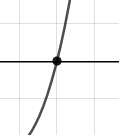
\includegraphics[width=0.3\textwidth]{../Figures/polyZeroBehaviorDC.png}
    \end{center}\begin{enumerate}[label=\Alph*.]
\begin{multicols}{2}
\item 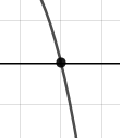
\includegraphics[width = 0.3\textwidth]{../Figures/polyZeroBehaviorAC.png}
\item 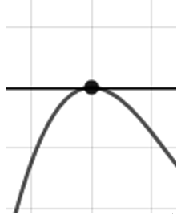
\includegraphics[width = 0.3\textwidth]{../Figures/polyZeroBehaviorBC.png}
\item 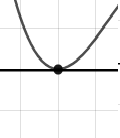
\includegraphics[width = 0.3\textwidth]{../Figures/polyZeroBehaviorCC.png}
\item 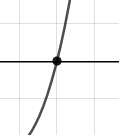
\includegraphics[width = 0.3\textwidth]{../Figures/polyZeroBehaviorDC.png}
\end{multicols}\item None of the above.\end{enumerate}
\textbf{General Comment:} You will need to sketch the entire graph, then zoom in on the zero the question asks about.
}
\litem{
Construct the lowest-degree polynomial given the zeros below. Then, choose the intervals that contain the coefficients of the polynomial in the form $x^3+bx^2+cx+d$.
\[ 5 - 2 i \text{ and } 1 \]The solution is \( x^{3} -11 x^{2} +39 x -29 \), which is option A.\begin{enumerate}[label=\Alph*.]
\item \( b \in [-14, -9], c \in [37, 44], \text{ and } d \in [-34, -23] \)

* $x^{3} -11 x^{2} +39 x -29$, which is the correct option.
\item \( b \in [2, 13], c \in [37, 44], \text{ and } d \in [27, 33] \)

$x^{3} +11 x^{2} +39 x + 29$, which corresponds to multiplying out $(x-(5 - 2 i))(x-(5 + 2 i))(x + 1)$.
\item \( b \in [-2, 6], c \in [-2, 5], \text{ and } d \in [-6, 1] \)

$x^{3} + x^{2} +x -2$, which corresponds to multiplying out $(x + 2)(x -1)$.
\item \( b \in [-2, 6], c \in [-6, -5], \text{ and } d \in [0, 8] \)

$x^{3} + x^{2} -6 x + 5$, which corresponds to multiplying out $(x -5)(x -1)$.
\item \( \text{None of the above.} \)

This corresponds to making an unanticipated error or not understanding how to use nonreal complex numbers to create the lowest-degree polynomial. If you chose this and are not sure what you did wrong, please contact the coordinator for help.
\end{enumerate}

\textbf{General Comment:} Remember that the conjugate of $a+bi$ is $a-bi$. Since these zeros always come in pairs, we need to multiply out $(x-(5 - 2 i))(x-(5 + 2 i))(x-(1))$.
}
\litem{
Which of the following equations \textit{could} be of the graph presented below?

\begin{center}
    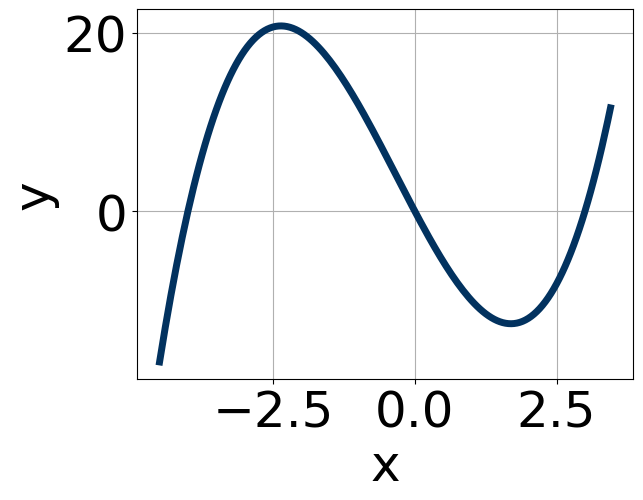
\includegraphics[width=0.5\textwidth]{../Figures/polyGraphToFunctionCopyC.png}
\end{center}


The solution is \( 7x^{9} (x + 4)^{11} (x - 3)^{9} \), which is option B.\begin{enumerate}[label=\Alph*.]
\item \( -11x^{6} (x + 4)^{11} (x - 3)^{5} \)

The factor $x$ should have an odd power and the leading coefficient should be the opposite sign.
\item \( 7x^{9} (x + 4)^{11} (x - 3)^{9} \)

* This is the correct option.
\item \( -6x^{7} (x + 4)^{5} (x - 3)^{5} \)

This corresponds to the leading coefficient being the opposite value than it should be.
\item \( 6x^{8} (x + 4)^{4} (x - 3)^{11} \)

The factors $0$ and $-4$ have have been odd power.
\item \( 8x^{8} (x + 4)^{5} (x - 3)^{7} \)

The factor $0$ should have been an odd power.
\end{enumerate}

\textbf{General Comment:} General Comments: Draw the x-axis to determine which zeros are touching (and so have even multiplicity) or cross (and have odd multiplicity).
}
\litem{
Describe the zero behavior of the zero $x = -8$ of the polynomial below.
\[ f(x) = 4(x - 7)^{5}(x + 7)^{3}(x + 8)^{9}(x - 8)^{8} \]The solution is the graph below, which is option D.
    \begin{center}
        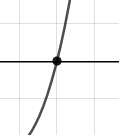
\includegraphics[width=0.3\textwidth]{../Figures/polyZeroBehaviorCopyDC.png}
    \end{center}\begin{enumerate}[label=\Alph*.]
\begin{multicols}{2}
\item 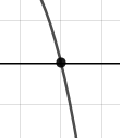
\includegraphics[width = 0.3\textwidth]{../Figures/polyZeroBehaviorCopyAC.png}
\item 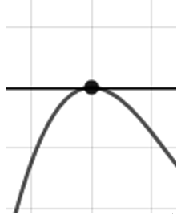
\includegraphics[width = 0.3\textwidth]{../Figures/polyZeroBehaviorCopyBC.png}
\item 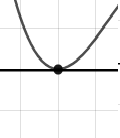
\includegraphics[width = 0.3\textwidth]{../Figures/polyZeroBehaviorCopyCC.png}
\item 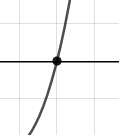
\includegraphics[width = 0.3\textwidth]{../Figures/polyZeroBehaviorCopyDC.png}
\end{multicols}\item None of the above.\end{enumerate}
\textbf{General Comment:} You will need to sketch the entire graph, then zoom in on the zero the question asks about.
}
\litem{
Which of the following equations \textit{could} be of the graph presented below?

\begin{center}
    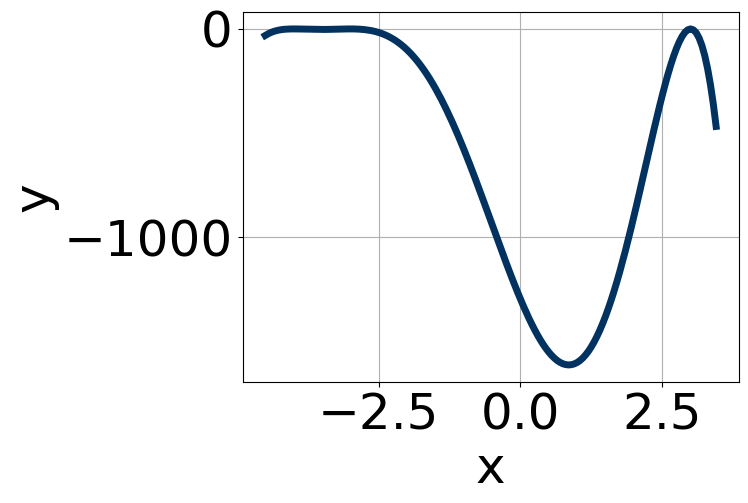
\includegraphics[width=0.5\textwidth]{../Figures/polyGraphToFunctionC.png}
\end{center}


The solution is \( -4(x + 4)^{4} (x - 3)^{10} (x + 3)^{4} \), which is option B.\begin{enumerate}[label=\Alph*.]
\item \( 16(x + 4)^{10} (x - 3)^{10} (x + 3)^{6} \)

This corresponds to the leading coefficient being the opposite value than it should be.
\item \( -4(x + 4)^{4} (x - 3)^{10} (x + 3)^{4} \)

* This is the correct option.
\item \( 14(x + 4)^{10} (x - 3)^{4} (x + 3)^{11} \)

The factor $(x + 3)$ should have an even power and the leading coefficient should be the opposite sign.
\item \( -7(x + 4)^{4} (x - 3)^{11} (x + 3)^{7} \)

The factors $(x - 3)$ and $(x + 3)$ should both have even powers.
\item \( -10(x + 4)^{10} (x - 3)^{6} (x + 3)^{11} \)

The factor $(x + 3)$ should have an even power.
\end{enumerate}

\textbf{General Comment:} General Comments: Draw the x-axis to determine which zeros are touching (and so have even multiplicity) or cross (and have odd multiplicity).
}
\litem{
Construct the lowest-degree polynomial given the zeros below. Then, choose the intervals that contain the coefficients of the polynomial in the form $x^3+bx^2+cx+d$.
\[ 5 - 2 i \text{ and } 4 \]The solution is \( x^{3} -14 x^{2} +69 x -116 \), which is option A.\begin{enumerate}[label=\Alph*.]
\item \( b \in [-17, -13], c \in [69, 79], \text{ and } d \in [-116, -115] \)

* $x^{3} -14 x^{2} +69 x -116$, which is the correct option.
\item \( b \in [-7, 5], c \in [-5, 6], \text{ and } d \in [-9, -2] \)

$x^{3} + x^{2} -2 x -8$, which corresponds to multiplying out $(x + 2)(x -4)$.
\item \( b \in [-7, 5], c \in [-13, -6], \text{ and } d \in [10, 27] \)

$x^{3} + x^{2} -9 x + 20$, which corresponds to multiplying out $(x -5)(x -4)$.
\item \( b \in [14, 16], c \in [69, 79], \text{ and } d \in [114, 119] \)

$x^{3} +14 x^{2} +69 x + 116$, which corresponds to multiplying out $(x-(5 - 2 i))(x-(5 + 2 i))(x + 4)$.
\item \( \text{None of the above.} \)

This corresponds to making an unanticipated error or not understanding how to use nonreal complex numbers to create the lowest-degree polynomial. If you chose this and are not sure what you did wrong, please contact the coordinator for help.
\end{enumerate}

\textbf{General Comment:} Remember that the conjugate of $a+bi$ is $a-bi$. Since these zeros always come in pairs, we need to multiply out $(x-(5 - 2 i))(x-(5 + 2 i))(x-(4))$.
}
\litem{
Describe the end behavior of the polynomial below.
\[ f(x) = -9(x + 2)^{4}(x - 2)^{5}(x - 6)^{5}(x + 6)^{7} \]The solution is the graph below, which is option A.
    \begin{center}
        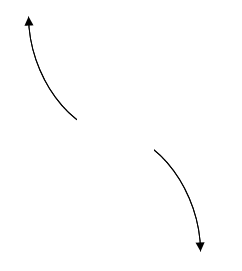
\includegraphics[width=0.3\textwidth]{../Figures/polyEndBehaviorCopyAC.png}
    \end{center}\begin{enumerate}[label=\Alph*.]
\begin{multicols}{2}
\item 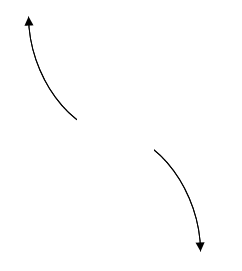
\includegraphics[width = 0.3\textwidth]{../Figures/polyEndBehaviorCopyAC.png}
\item 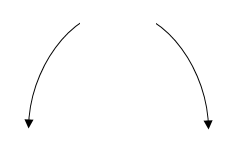
\includegraphics[width = 0.3\textwidth]{../Figures/polyEndBehaviorCopyBC.png}
\item 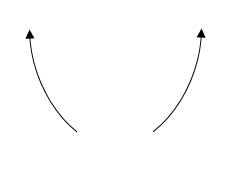
\includegraphics[width = 0.3\textwidth]{../Figures/polyEndBehaviorCopyCC.png}
\item 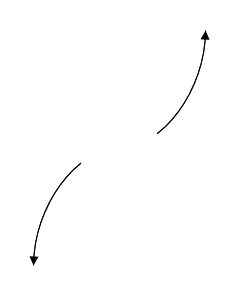
\includegraphics[width = 0.3\textwidth]{../Figures/polyEndBehaviorCopyDC.png}
\end{multicols}\item None of the above.\end{enumerate}
\textbf{General Comment:} Remember that end behavior is determined by the leading coefficient AND whether the \textbf{sum} of the multiplicities is positive or negative.
}
\litem{
Describe the end behavior of the polynomial below.
\[ f(x) = 9(x + 3)^{2}(x - 3)^{3}(x - 4)^{4}(x + 4)^{5} \]The solution is the graph below, which is option C.
    \begin{center}
        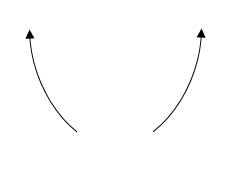
\includegraphics[width=0.3\textwidth]{../Figures/polyEndBehaviorCC.png}
    \end{center}\begin{enumerate}[label=\Alph*.]
\begin{multicols}{2}
\item 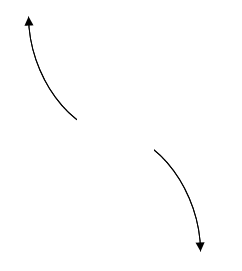
\includegraphics[width = 0.3\textwidth]{../Figures/polyEndBehaviorAC.png}
\item 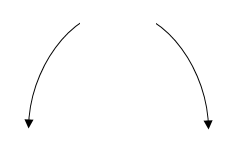
\includegraphics[width = 0.3\textwidth]{../Figures/polyEndBehaviorBC.png}
\item 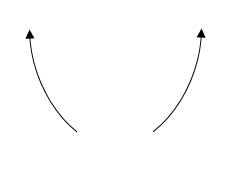
\includegraphics[width = 0.3\textwidth]{../Figures/polyEndBehaviorCC.png}
\item 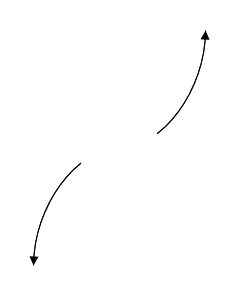
\includegraphics[width = 0.3\textwidth]{../Figures/polyEndBehaviorDC.png}
\end{multicols}\item None of the above.\end{enumerate}
\textbf{General Comment:} Remember that end behavior is determined by the leading coefficient AND whether the \textbf{sum} of the multiplicities is positive or negative.
}
\litem{
Construct the lowest-degree polynomial given the zeros below. Then, choose the intervals that contain the coefficients of the polynomial in the form $ax^3+bx^2+cx+d$.
\[ \frac{-7}{4}, \frac{-7}{5}, \text{ and } 4 \]The solution is \( 20x^{3} -17 x^{2} -203 x -196 \), which is option C.\begin{enumerate}[label=\Alph*.]
\item \( a \in [20, 23], b \in [-144, -139], c \in [301, 307], \text{ and } d \in [-196, -195] \)

$20x^{3} -143 x^{2} +301 x -196$, which corresponds to multiplying out $(4x -7)(5x -7)(x -4)$.
\item \( a \in [20, 23], b \in [9, 18], c \in [-207, -199], \text{ and } d \in [189, 200] \)

$20x^{3} +17 x^{2} -203 x + 196$, which corresponds to multiplying out $(4x -7)(5x -7)(x + 4)$.
\item \( a \in [20, 23], b \in [-19, -15], c \in [-207, -199], \text{ and } d \in [-196, -195] \)

* $20x^{3} -17 x^{2} -203 x -196$, which is the correct option.
\item \( a \in [20, 23], b \in [-92, -78], c \in [-26, -20], \text{ and } d \in [189, 200] \)

$20x^{3} -87 x^{2} -21 x + 196$, which corresponds to multiplying out $(4x -7)(5x + 7)(x -4)$.
\item \( a \in [20, 23], b \in [-19, -15], c \in [-207, -199], \text{ and } d \in [189, 200] \)

$20x^{3} -17 x^{2} -203 x + 196$, which corresponds to multiplying everything correctly except the constant term.
\end{enumerate}

\textbf{General Comment:} To construct the lowest-degree polynomial, you want to multiply out $(4x + 7)(5x + 7)(x -4)$
}
\end{enumerate}

\end{document}